\documentclass[letterpaper,12pt]{article}

\usepackage{threeparttable}
\usepackage{geometry}
\geometry{letterpaper,tmargin=1in,bmargin=1in,lmargin=1.25in,rmargin=1.25in}
\usepackage[format=hang,font=normalsize,labelfont=bf]{caption}
\usepackage{amsmath}
\usepackage{multirow}
\usepackage{array}
\usepackage{delarray}
\usepackage{amssymb}
\usepackage{amsthm}
\usepackage{lscape}
\usepackage{natbib}
\usepackage{setspace}
\usepackage{float,color}
\usepackage[pdftex]{graphicx}
\usepackage{pdfsync}
\usepackage{verbatim}
\usepackage{placeins}
\usepackage{geometry}
\usepackage{pdflscape}
\synctex=1
\usepackage{hyperref}
\hypersetup{colorlinks,linkcolor=red,urlcolor=blue,citecolor=red}
\usepackage{bm}


\theoremstyle{definition}
\newtheorem{theorem}{Theorem}
\newtheorem{acknowledgement}[theorem]{Acknowledgement}
\newtheorem{algorithm}[theorem]{Algorithm}
\newtheorem{axiom}[theorem]{Axiom}
\newtheorem{case}[theorem]{Case}
\newtheorem{claim}[theorem]{Claim}
\newtheorem{conclusion}[theorem]{Conclusion}
\newtheorem{condition}[theorem]{Condition}
\newtheorem{conjecture}[theorem]{Conjecture}
\newtheorem{corollary}[theorem]{Corollary}
\newtheorem{criterion}[theorem]{Criterion}
\newtheorem{definition}{Definition} % Number definitions on their own
\newtheorem{derivation}{Derivation} % Number derivations on their own
\newtheorem{example}[theorem]{Example}
\newtheorem{exercise}[theorem]{Exercise}
\newtheorem{lemma}[theorem]{Lemma}
\newtheorem{notation}[theorem]{Notation}
\newtheorem{problem}[theorem]{Problem}
\newtheorem{proposition}{Proposition} % Number propositions on their own
\newtheorem{remark}[theorem]{Remark}
\newtheorem{solution}[theorem]{Solution}
\newtheorem{summary}[theorem]{Summary}
\bibliographystyle{aer}
\newcommand\ve{\varepsilon}
\renewcommand\theenumi{\roman{enumi}}
\newcommand\norm[1]{\left\lVert#1\right\rVert}
\begin{document}

\subsection*{8.1}


Characteristic equations:
\[r_t=ae^{z_t}k_t^{\alpha-1}\]
\[c_t=e^{z_t}k_t^\alpha-k_{t+1}\]
\[c_t^{-1}=\beta E\{c_{t+1}^{-1}r_{t+1}\}\]
Steady states:
\[\bar{r}=\alpha\bar{k}^{\alpha-1}\]
\[1=\beta\bar{r}\]
\[\bar{c}=\bar{k}^\alpha-\bar{k}\]

Linearization and solving of $F, G, H, L,\& M$:
 \\ \\
\[F = \frac{\alpha \overline{K}^{\alpha-1}}{\overline{K}^{\alpha}-\overline{K}}\]
\[H = \frac{\alpha^2 \overline{K}^{2(\alpha-1)}}{\overline{K}^{\alpha}-\overline{K}}\]
\[G = -\frac{\alpha \overline{K}^{\alpha-1}(\alpha + \overline{K}^{\alpha-1})}{\overline{K}^{\alpha}-\overline{K}}\]
\[L = -\frac{\alpha \overline{K}^{2\alpha -1}}{\overline{K}^{\alpha}-\overline{K}}\]
\[P = \frac{-G \pm \sqrt{G^2-4FH}}{2F}\]
\[M = \frac{ \alpha^2 \overline{K}^{2(\alpha-1)}}{\overline{K}^{\alpha}-\overline{K}}\]
\[Q = -\frac{LN + M}{FN+FP+G}\] 
\\ 
and we get:
\[F = 2.38051966287\]
\[H = 1.68371931464\]
\[G = -5.16150615175\]
\[L = -1.6279703344\]
\[M = 1.68371931464\]
\[P = 0.83409605\]
\[ Q = 0.14998134\]
\\ 
Policy function:
\includegraphics[scale=0.7]{8_1}
Note that this is similar to the closed form solution.

\subsection*{8.2}


Characteristic equations:
\[c_t=e^{z_t}k_t^\alpha-k_{t+1}\]
\[c_t^{-1}=\beta E\{c_{t+1}^{-1}r_{t+1}\}\]
\[r_t=ae^{z_t}k_t^{\alpha-1}\]\\
Steady states:
\[\bar{c}=\bar{k}^\alpha-\bar{k}\]
\[1=\beta\bar{r}\]
\[\bar{r}=\alpha\bar{k}^{\alpha-1}\]
After linearizing,
\[\tilde{r}_t=z_t+(\alpha-1)\tilde{k}_t\]

\[\tilde{c}_t=-\frac{\bar{k}}{\bar{c}}\tilde{k}_{t+1}+\frac{\bar{k}^\alpha}{\bar{c}}\alpha\tilde{k}_t+\frac{\bar{k}^\alpha}{\bar{c}}z_t\]
\[\tilde{c}_t=E\{\tilde{r}_{t+1}\}-E\{\tilde{c_{t+1}}\}\]
Then we have that
\[F=\frac{\bar{k}^2}{\bar{c}}\]
\[G=\frac{\alpha\bar{k}^{\alpha+1}-\bar{k}^2}{\bar{c}}+(\alpha-1)\bar{k}\]
\[H=\frac{\alpha\bar{k}^{1+\alpha}}{\bar{c}}\]
\[L=\frac{\bar{k}-\bar{k}^{\alpha+1}}{\bar{c}}\]
\[M=\frac{\bar{k}^{1+\alpha}}{\bar{c}}\]
\\
and that
\[P=\frac{-G\underline{+}\sqrt{G^2-4FH}}{2F}\]
\[Q=-\frac{LN+M}{FN+FP+G}\]
Policy function:
\[\tilde{X}_t=(I_P)\bar{X}+P\tilde{X}_{t-1}+Q\tilde{z}_t\]
Numerical answers:
\[\bar{k}=.19278,\bar{r}=1.0204,\bar{c}=.36926,F=.100646,G=-4.8408,L=.22864,H=.102700,M=.293428, P=.486996, Q=.108734\]
\\
Policy function graphed:

\includegraphics[scale = .75]{8_2}

\subsection*{8.3}


\[E[F\tilde{X}_{t+1}+G\tilde{X_t}+H\tilde{X}_{t-1}+L\tilde{Z}_{t+1}+M\tilde{Z}_{t}] = 0\]
\[E[F(P\tilde{X_t})+G\tilde{Z}_{t+1}+L\tilde{Z}_{t+1}+M\tilde{Z_t}] = 0\]
\[E[(FP+G)\tilde{X_t}+H\tilde{X}_{t-1}+(FQ+L)\tilde{Z}_{t+1}+M\tilde{t}] = 0\]
\[E[(FP+G)(P\tilde{X}_{t-1}+Q\tilde{Z}_{t})+H\tilde{X}_{t-1}+(FG+L)(N\tilde{Z}_t+\varepsilon_{t+1})+M\tilde{Z_t}] = 0\]
\[= (FP^2+GP+H)\tilde{X}_{t-1}+(FPQ+GQ+FQN+LN+M)Z_t = 0\]
\[[(FP + G)P+H]\tilde{X}_{t-1}+[(FQ+L)N+(FP+G)Q+M]\tilde{Z}_t=0\]

\subsection*{8.4}



Steady state values:

$k=7.2875, c=1.4845, r=0.1215, w=1.3280, l=0.5797, T=0.0742, y=2.2133$ and $i=0.7287$
\\
\subsection*{8.5}



\begin{tabular}{lrrrrrrrr}
\hline
   &     $\bar{k}$ &   $\bar{c}$ &   $\bar{r}$ &   $\bar{w}$ &  $\bar{l}$ &   $\bar{T}$ & $\bar{y}$&  $\bar{i}$ \\
\hline
 $\delta$   & -48.345 &  -3.511 &  1     & -7.287 &  1.32  &  -0.176 &  -4.121 & -0.61  \\
 $\tau$  &  -2.323 &  -0.234 &  0.023 & -0.165 & -0.139 &   0.849 &  -0.467 & -0.232 \\
 $\bar{z}$ &   0     &   0     &  0     &  0     &  0     &   0     &   0.77  &  0     \\
 $\alpha$  &  25.986 &   2.085 &  0     &  4.396 & -0.769 &   0.104 &   4.684 &  2.599 \\
 $\gamma$  &   0.139 &   0.028 &  0     &  0     &  0.019 &   0.001 &   0.042 &  0.014 \\
 $\xi$   &  -0.802 &  -0.163 &  0     &  0     & -0.11  &  -0.008 &  -0.243 & -0.08  \\
 $\beta$ &  65.438 &   1.751 & -1.096 &  7.988 &  0.26  &   0.088 &   8.295 &  6.544 \\
 $a$ &  -1.849 &  -0.377 &  0     &  0     & -0.254 &  -0.019 &  -0.562 & -0.185 \\
\hline
\end{tabular}\\
\\\\
\subsection*{8.6}


We have that

\[F= \begin{bmatrix} 
2.9046023 & -3.74013067\\
  0.    &      0.    \\ 
  \end{bmatrix}\]
\[G=\begin{bmatrix}
-5.88765983 & 3.8571742 \\
  2.90460231 &-8.11672985\\ 
 \end{bmatrix}\]
\[H=\begin{bmatrix}
 2.96699945 & 0. \\      
 -2.87232918 & 0.\\   
 \end{bmatrix}\]
\[L=\begin{bmatrix} 
-2.1684962\\
 0.   \\ 
 \end{bmatrix}\]
\[M = \begin{bmatrix} 
 2.23635669\\
 -1.6363563\\
 \end{bmatrix}\]
\[P=\begin{bmatrix} 
0.9153012  & 0.\\
-0.02633366 & 0.\\
\end{bmatrix}\]
\[Q=\begin{bmatrix} 
0.54506616\\
 -0.00654893\\
 \end{bmatrix}\]
\subsection*{8.7}


Linearized policy function graph:\\
\includegraphics[scale = .75]{8_7}
\subsection*{8.8}


\includegraphics[scale = .60]{8_8_path}

\includegraphics[scale = .75]{8_8}

\subsection*{8.9}

\includegraphics[scale = .40]{8_9}

\subsection*{8.10}

\includegraphics[scale = .60]{8_10}

\subsection*{8.11}

Lower compuational time leads to a loss in accuracy.

\includegraphics[scale = .60]{8_11}

\includegraphics[scale = .60]{8_11a}

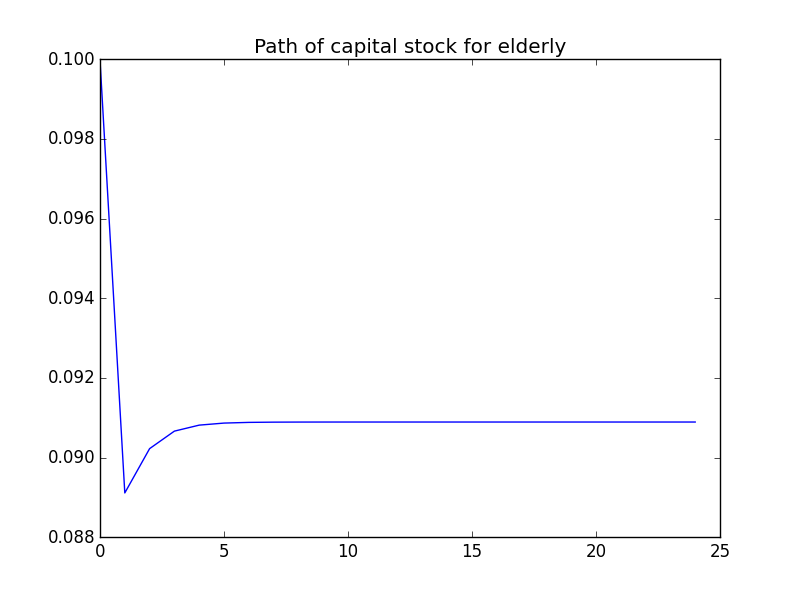
\includegraphics[scale = .60]{eightelevenc}


\subsection*{8.12}


\includegraphics[scale = .60]{8_12}

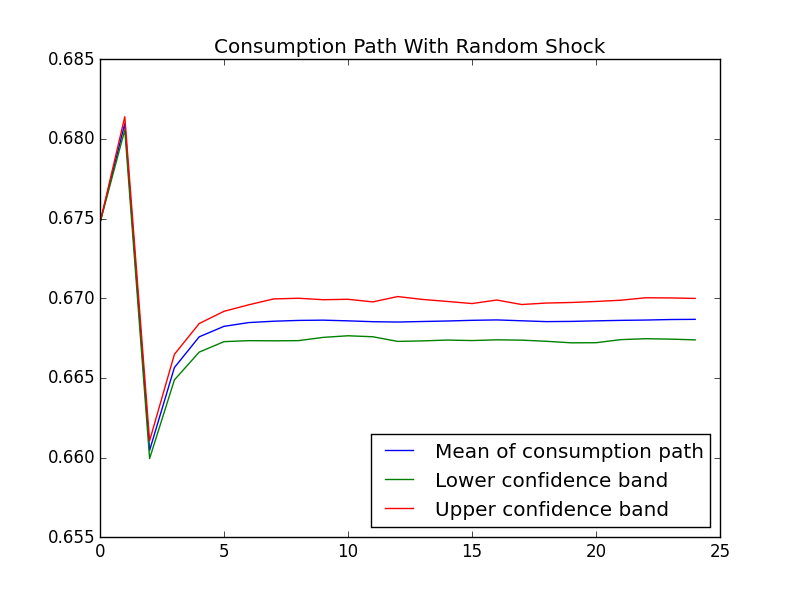
\includegraphics[scale = .60]{eighttwelveb}

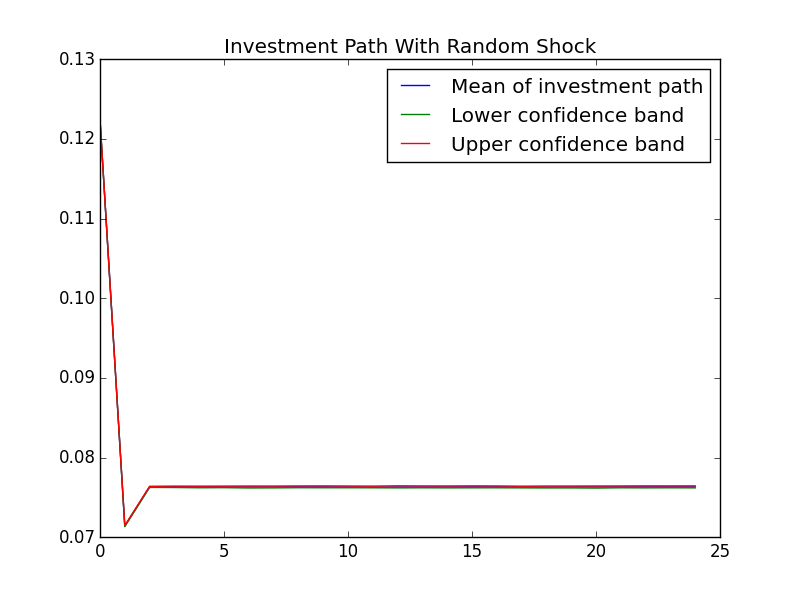
\includegraphics[scale = .60]{eighttwelvec}













\end{document}
